\chapter{Understanding Desire}

This chapter follows J. Krishnamurti's conversation with Dr. Alan W. Anderson on desire, pleasure, fear, and control. There is no blackboard mathematics in the source material, so the notation used here is a disciplined shorthand for the movement of the inquiry, not a formal psychological theory. The aim is to preserve the spoken order: fear first, then freedom, then pleasure, then the deeper question of desire, and only after that the question of control and the possibility of living without it.

\section{Fear, Pleasure, And Freedom}

Anderson begins from the previous conversation. Fear and pleasure had been called opposite sides of the same coin, and the natural question is whether we can now move from fear into pleasure. Krishnamurti does not take that step immediately. He first returns to fear, because fear has produced not merely private discomfort but whole structures of thought, belief, ideology, and gods.

The first precision is about freedom. We often speak as though freedom meant being free from something: free from fear, free from burden, free from conflict. But Krishnamurti makes a sharper distinction. Freedom from fear still has fear as its reference point. Freedom for an end still has direction, motive, and conflict built into it.

Let \(F\) denote freedom itself, and let \(F_{\mathrm{from}}(x)\) and \(F_{\mathrm{for}}(x)\) denote the movements of escape from an object and movement toward an object. The lecture's first conceptual distinction can be written as
\begin{equation}
F_{\mathrm{from}}(x) \neq F,
\qquad
F_{\mathrm{for}}(x) \neq F.
\end{equation}
This is only notation for the inquiry. The point is not that freedom has been mathematically defined. The point is that a movement away from fear is still a movement organized by fear.

\subsection{Question \& Answer}

\paragraph{Question.}
If one is free from fear, is that not freedom?

\paragraph{Answer.}
Not necessarily. To be free from fear may still mean that fear has shaped the problem and the desired outcome. Krishnamurti points instead to a freedom that is not ``from,'' not ``for,'' and not even ``in'' something. It is not reached by struggling against a burden; rather, the burden is no longer there. In that sense, relationship itself is seen in freedom, not as a project of escape.

\section{Inquiry Without Condemnation}

Only after this clearing does the dialogue return to pleasure. Pleasure and fear are not separable in life, Krishnamurti says, though they may be separated for investigation. Anderson hears the familiar connection: punishment and reward, fear and pleasure, the expectation of gratification and the nervousness of not receiving it.

The paired structure may be summarized as
\begin{equation}
\mathrm{Fear} \leftrightarrow \mathrm{Pleasure},
\qquad
\mathrm{Punishment} \leftrightarrow \mathrm{Reward}.
\end{equation}
The arrows do not mean a strict causal law. They mark a lived pairing: the mind that is trained by punishment is also trained by reward; the mind that seeks pleasure is also shadowed by fear.

Before the inquiry can proceed, Krishnamurti removes two common distortions. Pleasure is not to be condemned, and it is not to be justified. The lecture is not moving toward puritanism, permissiveness, or moral permission. It is trying to observe. That word matters: observation here means looking without the inclination to suppress, approve, defend, or pursue.

\begin{definition}
For this chapter, \emph{observation} means direct looking without condemnation, justification, acceptance, or suppression. It is not a method imposed on desire; it is the condition under which desire can be seen.
\end{definition}

\section{Why Pleasure Leads Back To Desire}

Anderson names the ordinary field of pleasure: anticipation, gratification, satisfaction, and fulfilment. Krishnamurti accepts the direction but says that to understand pleasure we must first look at desire. This is the first major turn in the lecture. Pleasure is not yet the center; desire is the movement beneath it.

In the social field, desire is not left alone. It is stimulated, nourished, expanded, and inflamed. Krishnamurti gives the examples of commercialism, consumerism, propaganda, fashion, and the demand for more. The fashion cycle matters because it shows a simple mechanism: pleasure fades, and therefore a stronger or newer stimulus is required.

As a cautious schematic, we can write
\begin{equation}
\mathrm{stimulation}
\longrightarrow D
\longrightarrow \mathrm{fulfilment}
\longrightarrow \mathrm{fading}
\longrightarrow \mathrm{stronger\ stimulus}.
\end{equation}
Here \(D\) denotes desire. This is not an economic model of consumer behavior. It is a compact way of preserving the lecture's movement: desire is inflamed by a world that knows how to stimulate it.

The same pattern appears in ritual. Words, chants, symbols, images, flowers, incense, color, and theatrical beauty can stimulate a particular appetite. Krishnamurti does not deny that such things may be beautiful. The point is subtler: when the stimulation becomes central, the listener may no longer be attending to what is being said or disclosed, but to the pleasure of the form.

\section{Appetite, Desire, And The Variable Object}

Anderson asks whether desire should be related to appetite and natural hunger. Krishnamurti says appetite and desire are related. There is physical appetite, psychological appetite, sexual appetite, intellectual appetite, and even appetite for ritual. The list is not a taxonomy for its own sake. It prepares the central distinction between the object desired and the movement of desire.

Let \(O_i\) denote an object of desire. It may be a house, a car, knowledge, God, enlightenment, sexual experience, power, ritual, or possession. Krishnamurti's point is that the objects vary, but the movement called desire remains.

\begin{equation}
O_i \ \hbox{varies},
\qquad
D \ \hbox{remains}.
\end{equation}

\begin{table}
\centering
\begin{tabular}{lll}
Object & Stimulus & Movement \\
Possession & coat, tie, house, car & desire to acquire \\
Knowledge & discussion, comparison & desire to accumulate \\
Ritual & chant, symbol, image & desire to be stimulated \\
God or truth & ideal, path, authority & desire transferred \\
Power & security, control & desire to secure pleasure
\end{tabular}
\end{table}

The table should not be read as a fixed classification. It simply gives a pocket-sized form to a repeated movement in the dialogue. One object may be called noble and another ignoble, but the lecture asks us to look behind that naming. If the same movement of desire is operating, the difference of object has not solved the problem.

\section{The Process Of Desire}

The lecture then asks the direct question: what is desire? Anderson first wonders whether desire is a sense of absence. Krishnamurti rejects that framing for the moment. He is not asking for an abstract definition. He is asking how desire comes about in each of us.

The transcript gives the process twice, with a small variation in order. First Krishnamurti says: visual perception, sensation, contact, and then desire. Anderson then recaps: visual perception, contact, sensation, desire. To avoid over-precision, we keep contact and sensation as a joined middle movement:
\begin{equation}
\mathrm{visual\ perception}
\longrightarrow
\mathrm{contact/sensation}
\longrightarrow
D.
\end{equation}
If desire is blocked, Anderson adds, anger follows; Krishnamurti accepts that all the rest follows. We may write the secondary movement as
\begin{equation}
D + \mathrm{frustration}
\longrightarrow
\mathrm{anger\ and\ further\ reaction}.
\end{equation}

\subsection{Question \& Answer}

\paragraph{Question.}
Is desire basically a sense of absence?

\paragraph{Answer.}
Krishnamurti does not take that route here. He asks us to observe the arising of desire rather than define it from a theory of lack. Something is seen; there is contact and sensation; desire comes out of that process. The important shift is from explaining desire in advance to watching its movement.

\begin{figure}
\centering
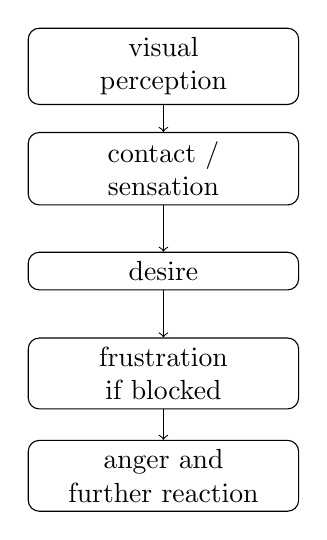
\begin{tikzpicture}[node distance=1.3cm]
\node[draw, rounded corners, align=center, text width=3.2cm] (a) {visual\\perception};
\node[draw, rounded corners, align=center, text width=3.2cm, below of=a] (b) {contact /\\sensation};
\node[draw, rounded corners, align=center, text width=3.2cm, below of=b] (c) {desire};
\node[draw, rounded corners, align=center, text width=3.2cm, below of=c] (d) {frustration\\if blocked};
\node[draw, rounded corners, align=center, text width=3.2cm, below of=d] (e) {anger and\\further reaction};
\draw[->] (a) -- (b);
\draw[->] (b) -- (c);
\draw[->] (c) -- (d);
\draw[->] (d) -- (e);
\end{tikzpicture}
\end{figure}

This diagram is a transcript-based reconstruction. It is not a board diagram. Its purpose is to make visible the sequence that the conversation names and then immediately uses.

\section{Control, Suppression, And The Loss Of Energy}

Once desire is seen, the historical answer appears: control it, suppress it, or transfer it to something higher. If desire causes trouble, dissipates energy, or exposes one to temptation, then the religious answer has often been to avoid contact with the world: do not look, do not expose yourself, keep reading the sacred book, hold the energy for God.

Krishnamurti turns this answer around. Control is not freedom from desire. Control is still organized by desire and fear. It narrows perception. It turns discipline into suppression. It may call itself religious, but its movement is still a reaction.

\begin{equation}
D
\xrightarrow{\mathrm{control/suppression/transfer}}
\mathrm{restriction}
+
\mathrm{loss\ of\ free\ energy}.
\end{equation}
The phrase ``free energy'' must be read in the language of the conversation, not as a physical quantity. It names the vitality that is squeezed out when the mind is occupied with suppressing, avoiding, and transferring desire.

\subsection{Question \& Answer}

\paragraph{Question.}
Need there be control of desire at all?

\paragraph{Answer.}
This is the problem Krishnamurti says arises once desire and appetite are seen. The usual answer is control; the lecture questions the whole structure of that answer. Control assumes that desire is to be mastered by an opposing force, but that opposition is itself conflict. The question is therefore not how to control desire more successfully, but whether desire can be understood so completely that the whole machinery of control is seen for what it is.

\begin{proposition}
If desire is merely transferred from one object to another, the movement of desire has not ended.
\end{proposition}

\begin{proof}
Let \(O_{\mathrm{worldly}}\) be an object such as money, possession, or status, and let \(O_{\mathrm{spiritual}}\) be an object such as God, truth, enlightenment, or heaven. If the object changes but the movement \(D\) remains a movement of acquisition, fulfilment, and becoming, then the substitution is structural rather than transformative:
\begin{equation}
D(O_{\mathrm{worldly}})
\sim
D(O_{\mathrm{spiritual}}).
\end{equation}
The symbol \(\sim\) marks similarity of movement, not formal equality. The lecture's practical conclusion is that changing the object does not by itself resolve desire.
\end{proof}

\section{The Cruelty Of Substitution}

The dialogue then becomes concrete. Krishnamurti tells of monks who avoided the sky, the trees, the water, and ordinary human beauty because they feared temptation. He tells of a young monk who had taken a vow of celibacy and resorted to an extreme physical act in the name of control. Anderson brings in Origen as a parallel case. Krishnamurti then speaks of others who tortured themselves for an idea, a symbol, or a concept.

These stories should be read with restraint. Their function is not shock. They show the logic of control carried into life. An idea of God, truth, or purity can become an object of desire; in pursuit of that object, the body and mind may be forced, narrowed, and damaged.

A second story deepens the same pattern. A man gives up his public role, spends twenty-five years meditating on truth, and later sees that he has been caught in his own verbal and intellectual structure. Another man spends fifty-five years going from teacher to teacher in search of God. Krishnamurti places this beside the business life of going to the office for fifty years in pursuit of money and things. The objects are different; the movement may be the same.

The working schema is therefore:
\begin{align}
\hbox{money, things, status} &\longrightarrow D,\\
\hbox{God, truth, enlightenment} &\longrightarrow D.
\end{align}
The point is not that these words name the same object. The point is that desire can put on sacred language without ceasing to be desire.

\section{Toward Pleasure, Enjoyment, And Joy}

After this long inquiry into desire, Krishnamurti returns to pleasure. The foundation is now in place. Unless appetite and desire are understood, pleasure cannot be understood deeply. Fear and pleasure remain paired principles, and reward and punishment remain their social expression.

The next precision concerns power. Anderson asks whether the search for power secures a pleasure not yet realized. Krishnamurti agrees. In this form, negating desire through power is itself another search. The mind says: I will control desire in order to secure a future state, a future pleasure, a future safety.

Society appears divided, but both sides are implicated. The religious side says control. Commercialism says enjoy, buy, sell. The human mind moves between them: pursue pleasure here, offer something to God there. Krishnamurti calls attention to this game because it has gone on for a very long time.

At the end, the vocabulary opens:
\begin{equation}
P,\quad E,\quad J,\quad H,
\end{equation}
where \(P\) is pleasure, \(E\) is enjoyment, \(J\) is joy, and \(H\) is happiness. Krishnamurti says joy is happiness, but he does not complete the full relation among the terms in this conversation. We should therefore keep the relation open:
\begin{equation}
J \approx H,
\qquad
P \ ? \ E \ ? \ J/H.
\end{equation}
The question mark is deliberate. The lecture does not close with a system; it opens a new step.

The last example is beauty. One sees a mountain, a lake, or a single tree on a hill. At that moment, Krishnamurti says, there is nothing but that. The beauty has knocked everything out of the observer. There is no division between me and that. There is purity and enjoyment. The chapter should stop there, because the conversation itself stops at the edge of the next inquiry: what takes place after that moment?

\section{Summary}

We have followed the lecture's order rather than imposing a finished theory on it. Fear first shows why freedom cannot be reduced to escape. Pleasure is then approached without condemnation, but the inquiry immediately turns toward desire. Desire is separated from its changing objects and traced through perception, contact, sensation, and reaction. Control appears as the traditional solution, but the lecture questions whether control is itself another form of conflict and substitution.

The compact form of the chapter is this:
\begin{align}
F_{\mathrm{from}}(x) &\neq F,\\
O_i \ \hbox{varies},\quad D &\ \hbox{remains},\\
\mathrm{visual\ perception} \to \mathrm{contact/sensation} &\to D,\\
D \xrightarrow{\mathrm{control}} \mathrm{restriction} &+ \mathrm{loss\ of\ free\ energy}.
\end{align}
The next inquiry will have to take up pleasure, enjoyment, joy, and happiness without losing what has just been seen: desire is not understood by condemning it, indulging it, or controlling it. It is understood, if at all, by looking at its movement directly.